\documentclass[11pt]{article}
\usepackage[a4paper,margin=1in]{geometry}
\usepackage{amsmath,amssymb,amsthm}
\usepackage{mathtools}
\usepackage[T1]{fontenc}
\usepackage{lmodern}
\usepackage{microtype}
\usepackage{tikz}
\usepackage{subcaption}

\newtheorem{theorem}{Theorem}
\newtheorem{lemma}{Lemma}
\definecolor{jobhighlight}{HTML}{9ABCE4}
\newcommand{\machinerow}[2]{%
    \node[machine, anchor=east] at (-0.3,-#1+0.5) {$M_{#2}$};
}

\newcommand{\dotsrow}[1]{%
    \foreach \dy in {-0.18,0,0.18} { % chktex 1
        \fill (-0.6,{-#1+0.5+\dy}) circle[radius=0.025];
        \fill (2,{-#1+0.5+\dy}) circle[radius=0.025];
    }
}

\newcommand{\jobblock}[5][white]{%
    \draw[job, fill=#1] (#3,-#2) rectangle ++(#4,1);
    \node at ({#3 + #4/2},{-#2 + 0.5}) {$#5$}; % chktex 1
}

\newcommand{\schedulemtwoone}{
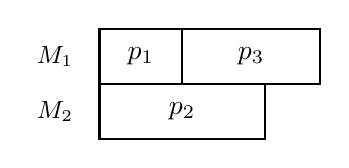
\begin{tikzpicture}[
    x=0.7cm,
    y=0.7cm,
    job/.style={
        draw,
        thick,
        fill=white,
        font=\small
    },
    machine/.style={font=\small}
]

% Displayed machine rows
\machinerow{1}{1}
\machinerow{2}{2}



% Edit the second schedule here.

\jobblock{1}{0}{1.5}{p_1}
\jobblock{1}{1.5}{2.5}{p_3}




\jobblock{2}{0}{3}{p_2}



\end{tikzpicture}
}

\newcommand{\schedulemtwotwo}{
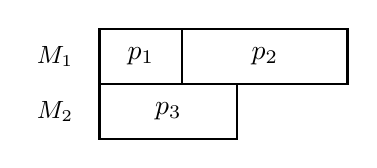
\begin{tikzpicture}[
    x=0.7cm,
    y=0.7cm,
    job/.style={
        draw,
        thick,
        fill=white,
        font=\small
    },
    machine/.style={font=\small}
]

% Displayed machine rows
\machinerow{1}{1}
\machinerow{2}{2}



% Edit the second schedule here.

\jobblock{1}{0}{1.5}{p_1}
\jobblock{1}{1.5}{3}{p_2}



\jobblock{2}{0}{2.5}{p_3}



\end{tikzpicture}
}

\begin{document}

\title{m=2 Upper Bound for the Case of One Job with Zero Processing Time}
\author{}
\date{}
\maketitle

\section*{Problem Statement for the case of \(OPT= (j_1, j_2 ; j_3)\)}

\begin{lemma}[m=2]

    The approximation ratio of the $\mathrm{WSPT}$-rule for $2||\sum_{j} w_j C^{\alpha}_j$ is

   \[
\lambda_{\alpha}
=
\begin{cases}
1+\dfrac{1}{2\alpha\left(1+\sqrt{3+\frac{1}{\alpha}}\right)},
& \alpha\in (0,\frac12],\\[1.2ex]
\infty,
& \alpha=0.
\end{cases}
\]
\end{lemma}
The proof of this can be found in the Appendix...


We know from ... and... that ... and ... hold. Thus, we can restrict ourself to instances with 
three jobs.
\begin{proof}
Let
\[
Q := p_1^2+p_3^2+p_2^2,
\]
and let \(\alpha\) be a parameter with \(0 \le \alpha \le \tfrac12\).
We want to maximize
\[
\frac{{(p_1+p_2)}^2+{(p_3)}^2+(2\alpha-1)Q}{{(p_1+p_3)}^2+{(p_2)}^2+(2\alpha-1)Q}
\]
over \(p_1,p_3,p_2 \ge 0\), subject to the following contraints:
\begin{align}
&p_3 \ge p_1\\
&p_3 \le p_2\\
&p_1 \le p_2.
\end{align}
These must hold so that the schedule actually is a list schedule.
\begin{figure}[htbp]
\centering
\setlength{\fboxsep}{6pt}
\fbox{%
\begin{minipage}{0.94\textwidth}
    \begin{minipage}[t]{0.47\linewidth}
        \centering
        \scalebox{0.8}{\schedulemtwoone}
        \par\smallskip
        \small(a) \(\sigma^{*}(I_1)\)
    \end{minipage}
    \hfill
    \begin{minipage}[t]{0.47\linewidth}
        \centering
        \scalebox{0.8}{\schedulemtwotwo}
        \par\smallskip
        \small(b) \(\sigma^{W}(I_1)\)
    \end{minipage}
\end{minipage}%
}
\caption{Schedules for $m=2$}
\label{figure-schedulecaseone}
\end{figure}

\section{Simplifying the objective}

We can rewrite the numerator
\begin{align*}
&{(p_1+p_2)}^2+{(p_3)}^2+(2\alpha-1)Q\\
&= (p_1^2+p_2^2+2p_1p_2)+(p_3^2)+(2\alpha-1)Q\\
&= 2p_1p_2 + 2\alpha Q.
\end{align*}
Similarly, the denominator becomes
\[
{(p_3+p_1)}^2+{(p_2)}^2+(2\alpha-1)Q = 2p_1p_3+2\alpha Q.
\]
Therefore
\[
\lambda_{\alpha}(I)
=
\frac{\alpha Q+p_1p_2}{\alpha Q+p_1p_3}=1+\frac{p_1(p_2-p_3)}{\alpha Q+p_1p_3}.
\]

We only gain over \(1\) when \(p_1(p_2-p_3)>0\).
So we may restrict our search to instances for which \(p_2>p_3\).

The restrictions read: \(p_1 \le p_3 \le p_2\)

\(\lambda_{\alpha}\) is monotonically decreasing in \(p_3\). 
We thus set \(p_3=p_1\) to maximize \(\lambda_{\alpha}\). 
This is consistent with the restriction \(p_1 \le p_3\).

\break
Our previous observation gives us the expression: 
\[
\max_{p_1,p_2\ge 0,\;p_2\ge p_1}
1+\frac{p_1(p_2-p_1)}{\alpha(2p_1^2+p_2^2)+p_1^2},
\qquad 0<\alpha\le \frac12.
\]

Set
\[
x=\frac{p_2}{p_1}.
\]
For \(p_1>0\), the restriction \(p_2\ge p_1\) becomes \(x\ge 1\), and
\[
1+\frac{p_1(p_2-p_1)}{\alpha(2p_1^2+p_2^2)+p_1^2}
=
1+\frac{x-1}{\alpha(2+x^2)+1}.
\]
Thus we maximize
\[
f(x)=1+\frac{x-1}{\alpha x^2+2\alpha+1},
\qquad x\ge 1.
\]

The derivative is
\[
f'(x)
=
\frac{\alpha x^2+2\alpha+1-2\alpha x(x-1)}
{{(\alpha x^2+2\alpha+1)}^2}
\]
and therefore
\[
f'(x)
=
\frac{-\alpha x^2+2\alpha x+2\alpha+1}
{{(\alpha x^2+2\alpha+1)}^2}.
\]

The denominator is positive for \(0<\alpha\le \frac12\), so the critical points are determined by
\[
-\alpha x^2+2\alpha x+2\alpha+1=0.
\]

Which has the solutions
\[
x
=
1\pm \sqrt{3+\frac1\alpha}.
\]
Since \(x\ge 1\), only
\[
x^*=1+\sqrt{3+\frac1\alpha}
\]
is relevant.
This is a maximum, since  
\[
g(x):=-\alpha x^2+2\alpha x+2\alpha+1.
\]
is downward-opened parabola.


Thus the maximum is attained for all \(p_1>0\) with
\[
\boxed{
p_2=p_1\left(1+\sqrt{3+\frac1\alpha}\right) \quad \text{and} \quad p_3=p_1
}
\]
and the maximum excess over (1) is
\[
\boxed{
f(x^*)
=
\frac{1}{2\alpha\left(1+\sqrt{3+\frac1\alpha}\right)}
}.
\]

If \(\alpha=0\), then
\[
\frac{p_1(p_2-p_1)}{p_1^2}
=
\frac{p_2}{p_1}-1,
\]
which is unbounded above as \(p_2/p_1\to\infty\). Thus for \(\alpha=0\), no finite maximum exists.

Consequently, the maximal value of the original ratio is
\[
\boxed{
\lambda_{\alpha}
=
\begin{cases}
1+\dfrac{1}{2\alpha\left(1+\sqrt{3+\frac1\alpha}\right)},
    & 0<\alpha\le \dfrac12,\\[1.2ex]
+\infty,
    & \alpha=0.
\end{cases}
}.
\]
\end{proof}
\end{document}
